%% 
%% Copyright 2019-2020 Elsevier Ltd
%% 
%% This file is part of the 'CAS Bundle'.
%% --------------------------------------
%% 
%% It may be distributed under the conditions of the LaTeX Project Public
%% License, either version 1.2 of this license or (at your option) any
%% later version.  The latest version of this license is in
%%    http://www.latex-project.org/lppl.txt
%% and version 1.2 or later is part of all distributions of LaTeX
%% version 1999/12/01 or later.
%% 
%% The list of all files belonging to the 'CAS Bundle' is
%% given in the file `manifest.txt'.
%% 
%% Template article for cas-sc documentclass for 
%% single column output.

%\documentclass[a4paper,fleqn,longmktitle]{cas-sc}
\documentclass[a4paper,fleqn]{cas-sc}

%\usepackage[numbers]{natbib}
%\usepackage[authoryear]{natbib}
\usepackage[authoryear,longnamesfirst]{natbib}

\begin{document}
\let\WriteBookmarks\relax
\def\floatpagepagefraction{1}
\def\textpagefraction{.001}
\shorttitle{FracG}
\shortauthors{Kelka et~al.}
%\begin{frontmatter}

\title [mode = title]{FracG - An automated framework for discontinuity network characterization}                      
\tnotemark[1,2]

\tnotetext[1]{This research was conducted as part of the CSIRO Deep Earth Imaging Future Science Platform}

\author[1]{Ulrich Kelka}[]
\cormark[1]
\ead{uli.kelka@csiro.au}
\ead[url]{https://research.csiro.au/dei/people/ukelka/}
\credit{Conceptualization of this study, Methodology, Software, Data curation, Writing - Original draft preparation}
\address[1]{}

\author[1]{Stefan Westerlund}[]
\credit{Methodology, Software, Data curation, Writing - Original draft preparation}
\address[2]{}

\author[2]{Luk Peeters}[]
\credit{Data curation, Writing - Original draft preparation}
\address[2]{}
\cortext[cor1]{Corresponding author}

\begin{abstract}
This template helps you to create a properly formatted \LaTeX\ manuscript.

\noindent\texttt{\textbackslash begin{abstract}} \dots 
\texttt{\textbackslash end{abstract}} and
\verb+\begin{keyword}+ \verb+...+ \verb+\end{keyword}+ 
which
contain the abstract and keywords respectively. 
Each keyword shall be separated by a \verb+\sep+ command.
\end{abstract}

\begin{highlights}
\item Automatic discontinuity network characterization
\item Statistical description of fault and fracture networks
\item Assessment of fluid flow direction
\end{highlights}

\begin{keywords}
fault network \sep fracture network \sep statistical description \sep network analysis 
\end{keywords}

%Figure X: y- distance, spurs, repair, terminology, sinuosity
%Figure X: Explain properties of shape file ()
%Figure X: show graph algorithms on synthetic data

\maketitle

\section{Introduction}
The empirical description of topology and geometry of fault and fracture networks is an essential step in any investigation of the material properties of faulted and fractured media. The mechanical properties of fractured media such as stiffness or bulk rock strength differ significantly depending on the abundance of discontinuities. Rock stability is especially affected by the heterogeneity of fractures. Therefore, the analysis of the spatial arrangement of discontinuities allows for assessment of mechanical resilience and stability, for instance in underground mines~\citep{Wang2017, Kong2019}. Furthermore, the characterization of fault and fracture networks represents a critical step in evaluating reservoir quality~\citep{Bauer2017} and assessing fluid flow properties~\citep{Lopez1995, Gudmunsson2000}.

While faults and fractures are three dimensional discontinuities, we often rely on two-dimensional data as 3D datasets are difficult and too costly to obtain. Widely applicable characterizations of discontinuity patterns should therefore be based on the frequently available 2D trace maps. Depending on the area of interest (i.e. drill core, outcrop, or reservoir), the size of features to be analysed can range from millimetres up to several kilometres. Especially when considering the generic architecture of fault zones that comprises of a macroscopic core that is surrounded by an arrangement of mesoscopic features in the damage zone~\citep{Faulkner2010, Sutherland2012} the need for an analysis across scales becomes evident.

Key geometric properties of faults and fracture traces are their orientation, length, and sinuosity. The spatial arrangement can be characterized by determining density, intensity, and spacing, while the topological characterization assesses the connectivity and continuity~\citep{Sanderson2015}. The fractal geometry of the entire trace map, of the single lineaments as well as of the lineament centres and intersection points, can provide additional information on the spatial arrangement and the topology of the network~\citep{Roy2007}. 

Here we present an automated framework for 2D lineament analysis to characterize geometry, spatial arrangement, and topology. Geometric parameters are investigated in a statistical manner with maximum likelihood fitting to length distribution, and kernel density estimation of the principal orientations. In addition to the geometric properties, the spatial arrangement of the network is investigated, we apply window sampling to obtain densities, intensities, lineament centre to lineament centre spacing for the 2D datasets, and a classification of the spatial arrangement is obtained via box counting. 

As density, intensity, and box counting dimension yield limited information on the topology we utilize a graph representation to quantify the connectivity of the network and characterize it in terms of the percolation threshold~\citep{Sanderson2018}. After converting the network into a graph, classical graph algorithms such as shortest path and maximum flow can be applied to further assess the fluid flow properties of the network. In addition to the analysis, the vector data forms the input for generating a finite element mesh on which detailed fluid flow simulations can be performed.
The objectives of this contribution are: (i) introducing and testing an automatic data extraction tool for network analysis, (ii) demonstrate its performance on synthetic data, and (iii) showcase analysis of regional scale fault networks in South Australia.

\section{Fault and Fracture Analysis}
Fault and fracture analysis investigate the geometric properties, the spatial arrangement, and the topology of discontinuities in a network. The results can be utilized in hydrogeology~\citep{Partsinevelou2011}, reservoir characterization~\citep{Olson2009, Abbasi2020}, disposal systems for nuclear waste~\citep{Reeves2012, Tsang2015}, and can form the input for discrete fracture network models~\citep{Miyoshi2018}. Often the acquired data is analysed to obtain statistical distributions and relationships between parameters~\citep[and references therein]{Zeeb2013}. Upscaling of parameters can be performed to assess overall physical properties of larger scales (e.g. equivalent permeabilities). Scaling relationships between certain parameters such as length and displacements in faults or length and aperture in fractures allow for obtaining additional information based on the statistical analysis of discontinuity sets. In the following we brief the key areas of the analysis: geometric properties, spatial arrangement, and topology.

\subsection{Geometric Properties}
Geometric properties refer to orientation, length distribution, and sinuosity of the components building up the network. The principal orientations of lineaments are related to stress states acting on the system whereas faults or fractures that form in a unique stress state are forming one group. Note that this is only valid for non-conjugate (orthogonal) features and the entire discontinuity network is often a result of all stress states that acted on the system~\citep{Maerten2016, Lei2018}. The distribution of orientation in a network is therefore loosely related be to the number, intensity, and sequence of deformation events.

The length distribution in natural discontinuity networks is found to follow either a log-normal, an exponential, or a power-law distribution~\citep{Zeeb2013, Healy2017}. This is an essential parameter as the conductivity and storage are closely related to the length of a fracture, and the width of the damage zone scales with the length of a fault. These relationships are based on the correlation of length and displacement in faults~\citep{Gudmundsson2013} and the scaling between aperture and length in fractures~\citep{Renshaw1997, Mayrhofer2019}.

The sinuosity of a fault trace that can be observed on the surface is related to the stiffness (Young modulus) of the host rock and to the linkage between individual fault segments. Pronounced sinuosities of fault points towards heterogenic stiffness along strike~\citep{Bridwell1975} and/or successive linkage of individual segments~\citep{vonHagke2019}. 

\subsection{Spatial arrangement}
The patterns of fault or fracture networks impact earthquake hazards, fluid flow properties, and resilience of rock masses, and their characterization requires several approaches~\citep{Laubach2018, Laubach2018b}. Analysing the spatial arrangement helps in quantifying the structural heterogeneity or anisotropy that governs permeability, resilience, and seismic properties of rock masses (cite). The major quantities of interest are density, intensity~\citep{Rohrbaugh2002, Zeeb2013, Watkins2015}, spacing~\citep{Zusa2017}, and fractal dimension~\citep{Bour1999, Wilson2000, Wilson2001}.

Density and intensity are measures of the total frequency or cumulative length per unit area~\citep{Rohrbaugh2002, Zeeb2013, Watkins2015} whereas high density values point towards structural complex zones which can represent areas comprising an enhanced vertical fluid flow component~\citep{Dimmen2017}. 

The spacing of discontinuities in an array is proposed to be a function of strength and stress state, and the mechanical thickness of the faulted layer~\citep{Soliva2006, Zusa2017, Yang2020}. This measure helps to further quantify the heterogeneity of fault and fracture networks.

The abundance of faults and fractures across a wide range of scales may indicate that discontinuity pattern geometry is fractal~\citep[and references therein]{Bour1999}. One of the first attempts in describing the scale-invariance of natural fault systems was based on data obtained from the San Andreas fault and postulated a single parameter as governing the behaviour of the system, the fractal dimension $D-f$~\citep{Turcotte1986}. The fractal dimension can be considered as a metric for the characterization of the spatial arrangement of discontinuity networks~\citep{Walsh1993, Idziak1996, Roy2007} but should be accompanied by other geometrical  measures such as exponent of the length distribution~\citep{Bonnet2001}. A scaling relationship between the fractal dimension $D_f$ and the exponent of the length distribution $a$ was found to exist~\citep{Bour1999}. The fractal geometry can help to quantitatively (describe?) size scaling and spatial clustering in fracture networks, which is crucial for predicting the hydrological and mechanical properties of fractured rock masses~\citep{Barton1995, Liu2017}.  

\subsection{Topology}
In contrast to the purely geometrical parameters such as length, orientation and spacing, which can be expressed in physical units, topology is an abstract way of analysing the relationship and arrangement of objects in space. In networks, the measures of topology classify connectivity and sparsity of models~\citep{Kincaid2011}.

The topological network analysis of natural discontinuity networks yields information on the partition of the solid into separated blocks (Husby et al., 1997) and on the connectivity~\citep{Andresen2013}. Topology represents a dimensionless measure of connectivity and arrangement of natural discontinuity networks where the objects are represented as the edges and vertices of a graph~\citep{Morley2016, Sanderson2019}. In recent years the applicability of topological network analysis to fault and fracture networks has gained interest~\citep{Sanderson2019, Nyberg2019} as the information on connectivity is directly related to fluid flow properties and permeability of natural networks~\citep{Manzocchi2002, Renard2013}.

In addition to assessing flow properties, the topology of discontinuity networks also represents a metric that helps characterizing types of fault and fracture arrays~\citep{Morley2016}. As the number of intersections in a network that results from a sequence of different deformation events is generally larger that in single-phase deformation, topographical concepts also yield information on the development of an arrangement of faults~\citep{Duffy2017}.

\subsection{Existing software}
We would be remiss should we not mention the existing commercial and open-source software packages for fault and fracture analysis. A well-established commercial tool is |textsc{fracman}  which allows for analysis and modelling of fracture networks~\citep{Fracman2011}. A variety of open-source frameworks for fracture analysis exist and we name a few of the latest: for acquisition and processing of digital outcrop data, Digifract was is built on top of QGIS~\citep{Hardebol2013}.  FraNep is an Excel$^{TM}$ based tool written in Microsoft Visual Basic$^{TM}$ for statistical evaluation of 2D fracture networks~\citep{Zeeb2013}. A Matlab toolbox for fracture pattern quantification is FracPAQ~\citep{Healy2017}. One of the latest contributions to open-source fault and fracture analysis is the ArcGIS toolbox NetworkGT~\citep{Nyberg2018}. Our approach to topological characterization is mainly based on the work of~\citep{Sanderson2018, Sanderson2019}and therefore comparable to~\citep{Nyberg2018}.

\section{FracG workflow}
Our framework utilizes the gdal library~\citep{Gdal2018} for handling geospatial data, boost libraries for the geometrical~\citep{Gehrels2016} and topological analysis~\citep{Siek2001},the GNU Scientific Library (GSL) is utilized for statistic and mathematical analysis~\citep{Gough2009}, and automatic 2D finite mesh generation is realized by using gmsh API~\citep{Gehrels2016}. As the statistical analysis of large discontinuity networks that are for instance obtained by unmanned aerial vehicles (UAV) can be computationally expensive. We therefore choose C++ as the programming environment and parallized the most demanding part of the analysis with openMP~\citep{Dagum1998}. 

The network analysis is based on reading in an ESRI Shapefile containing lineament locations in a projected coordinate system. Note that geographic coordinate systems are currently not supported and the user will have to reproject his data into an projected reference system prior to the analysis. A gneric workflow of a complet anlysis also including rater data is outlined in figure ~\ref{fig02}. 

\begin{figure}[h]
\centering
	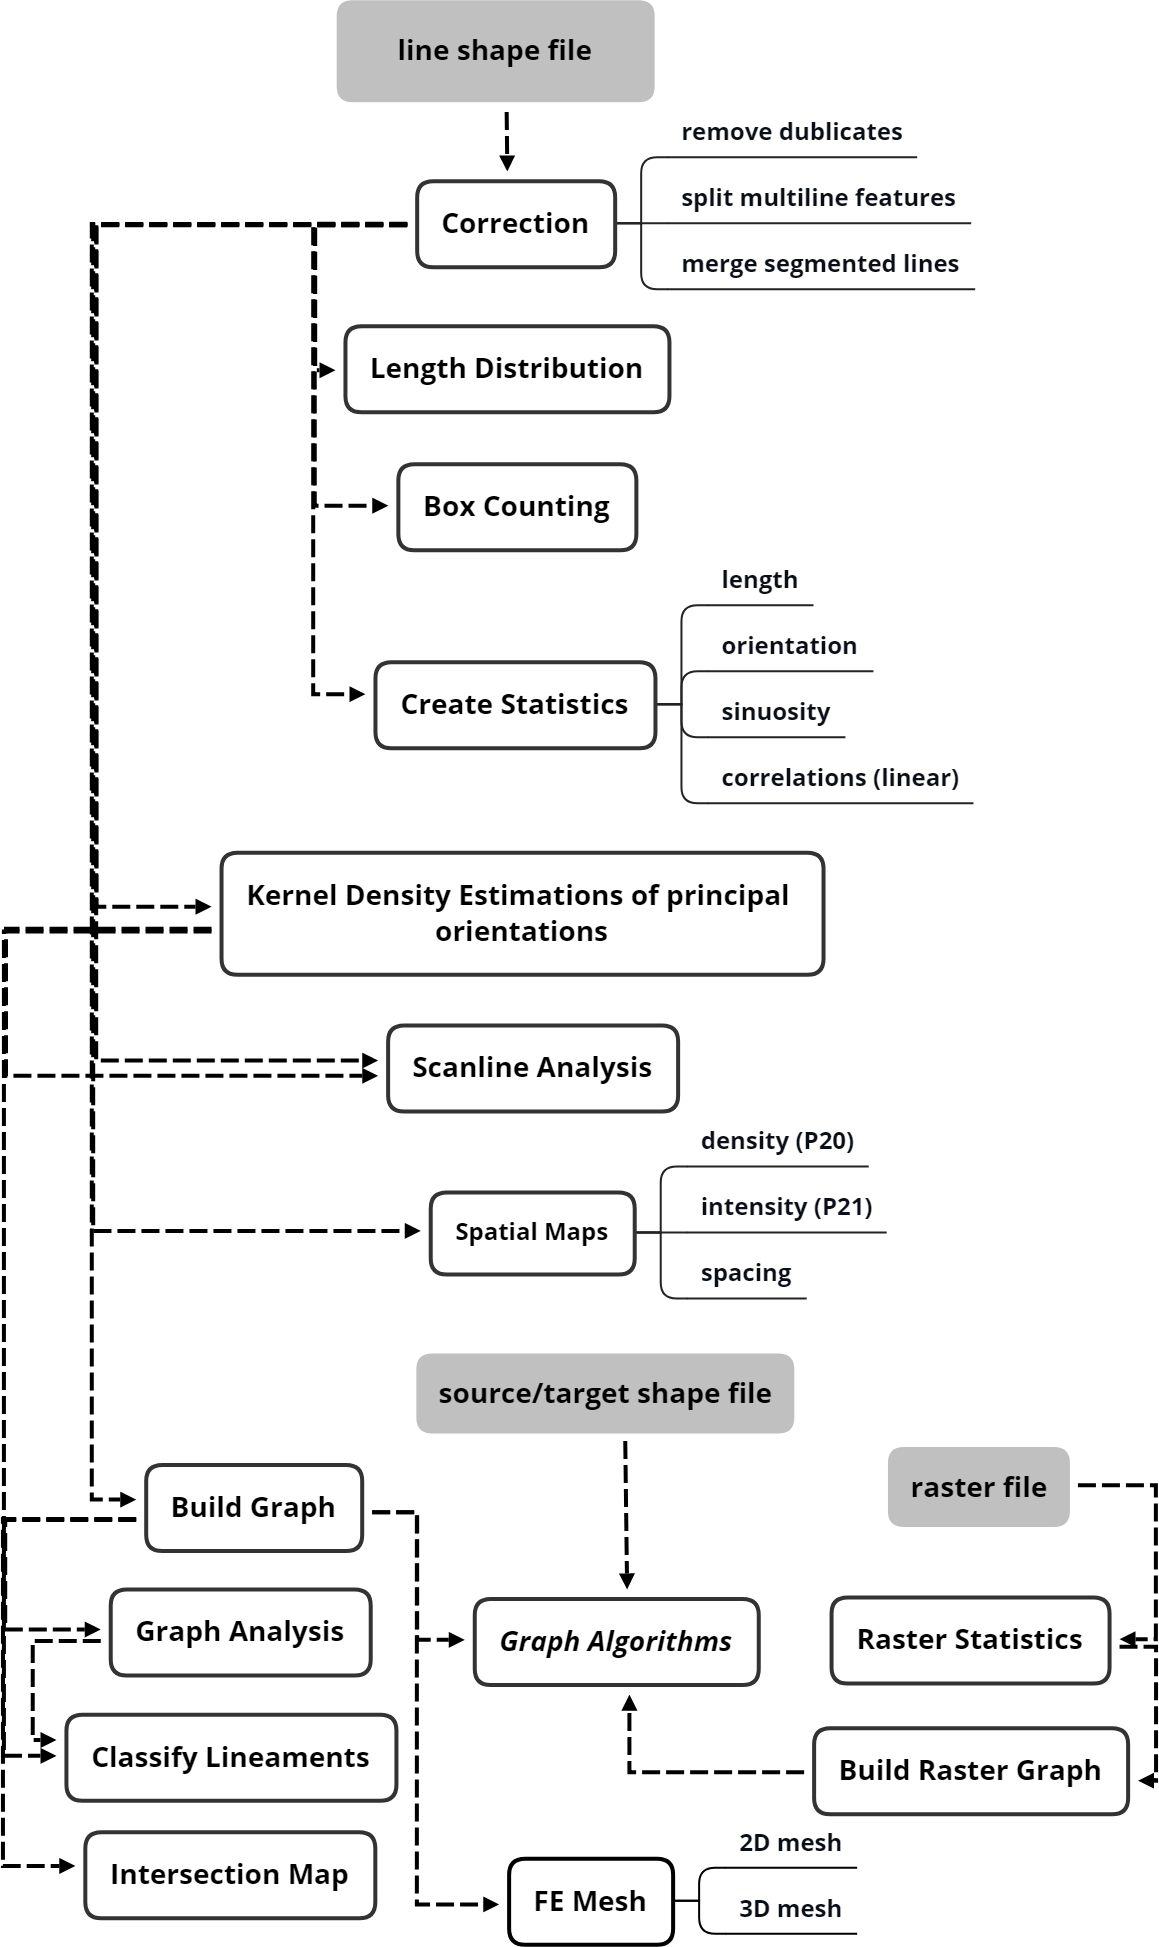
\includegraphics[width=8.5cm]{fig01.jpg}
	\caption{Schematic work flow of \textit{FracG} showing the different possible analysis. Grey shaded boxes represent data that needs to be passed to the program, the other boxes represent the different function s with associated outputs or performed tasks. The dotted arrows indicate  how the analysis progresses from initial input to the different products and how the respective functions are interlinked.}
\label{fig01}
\end{figure}

\subsection{Data import and correction}
Data on geological faults often represents a compilation of different datasets where the compiled data frequently exhibits flaws that would prevent reliable analysis of geometric properties. Therefore, the first step after importing the data format is to correct these flaws. After checking for a projected coordinate system, the data is read in and multi-lines are split into individual features. The subsequent step is the correction of the data is to merge falsely segmented lineaments. The features are merged based on a user-defined threshold representing the maximum distance between line-tips, and a maximum difference in orientation between adjacent line features is set to a user-defined range . This step often significantly reduces the number of separate digitized discontinuities and is crucial for performing reliable statistical analysis. After the correction the lineament set is also checked for potential duplicates and the corrected data can be written into a shape file.

\section{Geometrical Analysis}
We investigate the distributions of length, orientation, and sinuosity. At the current stage, the analysis is performed in Cartesian coordinates allowing for quick calculations but limiting the spatial accuracy for large scale data, for instance on a continental scale.

\subsection{Length distribution}
We obtain a statistical model for the length distribution and determine whether the data follows an exponential, log-normal, or a power-law distribution. We adapted the methods of~\citep{Clauset2009} for this problem the reader is referred to that work for further details. In the following we brief the general approach to obtaining the best fit of the empirical to a specific model:

First, we derive the model parameters for each distribution by maximum-likelihood methods and calculate the Kolmogorov-Smirnov (\textit{KS}) statistic between the data and each model. For each model, it is possible that there is a minimum value in the empirical distribution such that it is only accurately described by the statistical model above that minimum value. Such a minimum cut-off is chosen by determining the model parameters and evaluating the \textit{KS} statistic for each data point in the distribution and selecting the point with the minimum \textit{KS} statistic.

The suitability of the model for describing the empirical data is determined by comparing the \textit{KS} statistic of the model and data, against the \textit{KS} statistics calculated comparing sample distributions randomly drawn from the model and the new model which is generated from that random sample. In order to capture the characteristics of the original distribution, sample data points are drawn from either the candidate model or the below-minimum values of the empirical dataset, with a probability equal to the portion of the data points in the dataset that are above the minimum cut-off.

The number of samples, and therefore executions of the following steps, is derived from the maximum error (\textit{err}) we allow for out \textit{p}-value metric as:

\begin{equation}
	N=\frac{1}{4}err^2
\end{equation}

By this procedure, synthetic datasets of the same size as the original data are generated and the model parameters are derived from this synthetic dataset via maximum-likelihood estimates. We count the number of random sample distributions that result in a \textit{KS} value that is larger than the \textit{KS} value of the original dataset as \textit{c}. The \textit{p}-value that determines whether a model will be rejected is derive from this counter as:

\begin{equation}
	p=\frac{c}{N}
\end{equation}

Higher \textit{p}-values suggest that the model fits the data better. If there is more than one acceptable model, we proceed to determining which distribution fits the empirical data best. The goodness-of-fit is tested via pairwise log-likelihood comparisons of the candidate models. The minimum datapoint used in this comparison is the largest minimum value of the two distributions being compared. The log-likelihood ratio (\textit{R}) is calculated to determine which model is the better fit (table 1). We determine the reliability of this comparison using a second \textit{p}-value type, calculated here as:

\begin{equation}
	p = erfc \left( \frac{|R|}{\sqrt{2N}} \right)
\end{equation}

Here a lower value suggests more reliable comparison, and we consider the threshold for a meaningful comparison to be 0.1 After this procedure we report the type and parameters of the distribution(s) that best fit the empirical data.

In figure~\ref{fig03} we demonstrate the automatic fitting based on randomly created data synthetic data that follows an exponential (a), a log-normal (b) and a power law distribution(c).

\begin{figure}[h]
\centering
	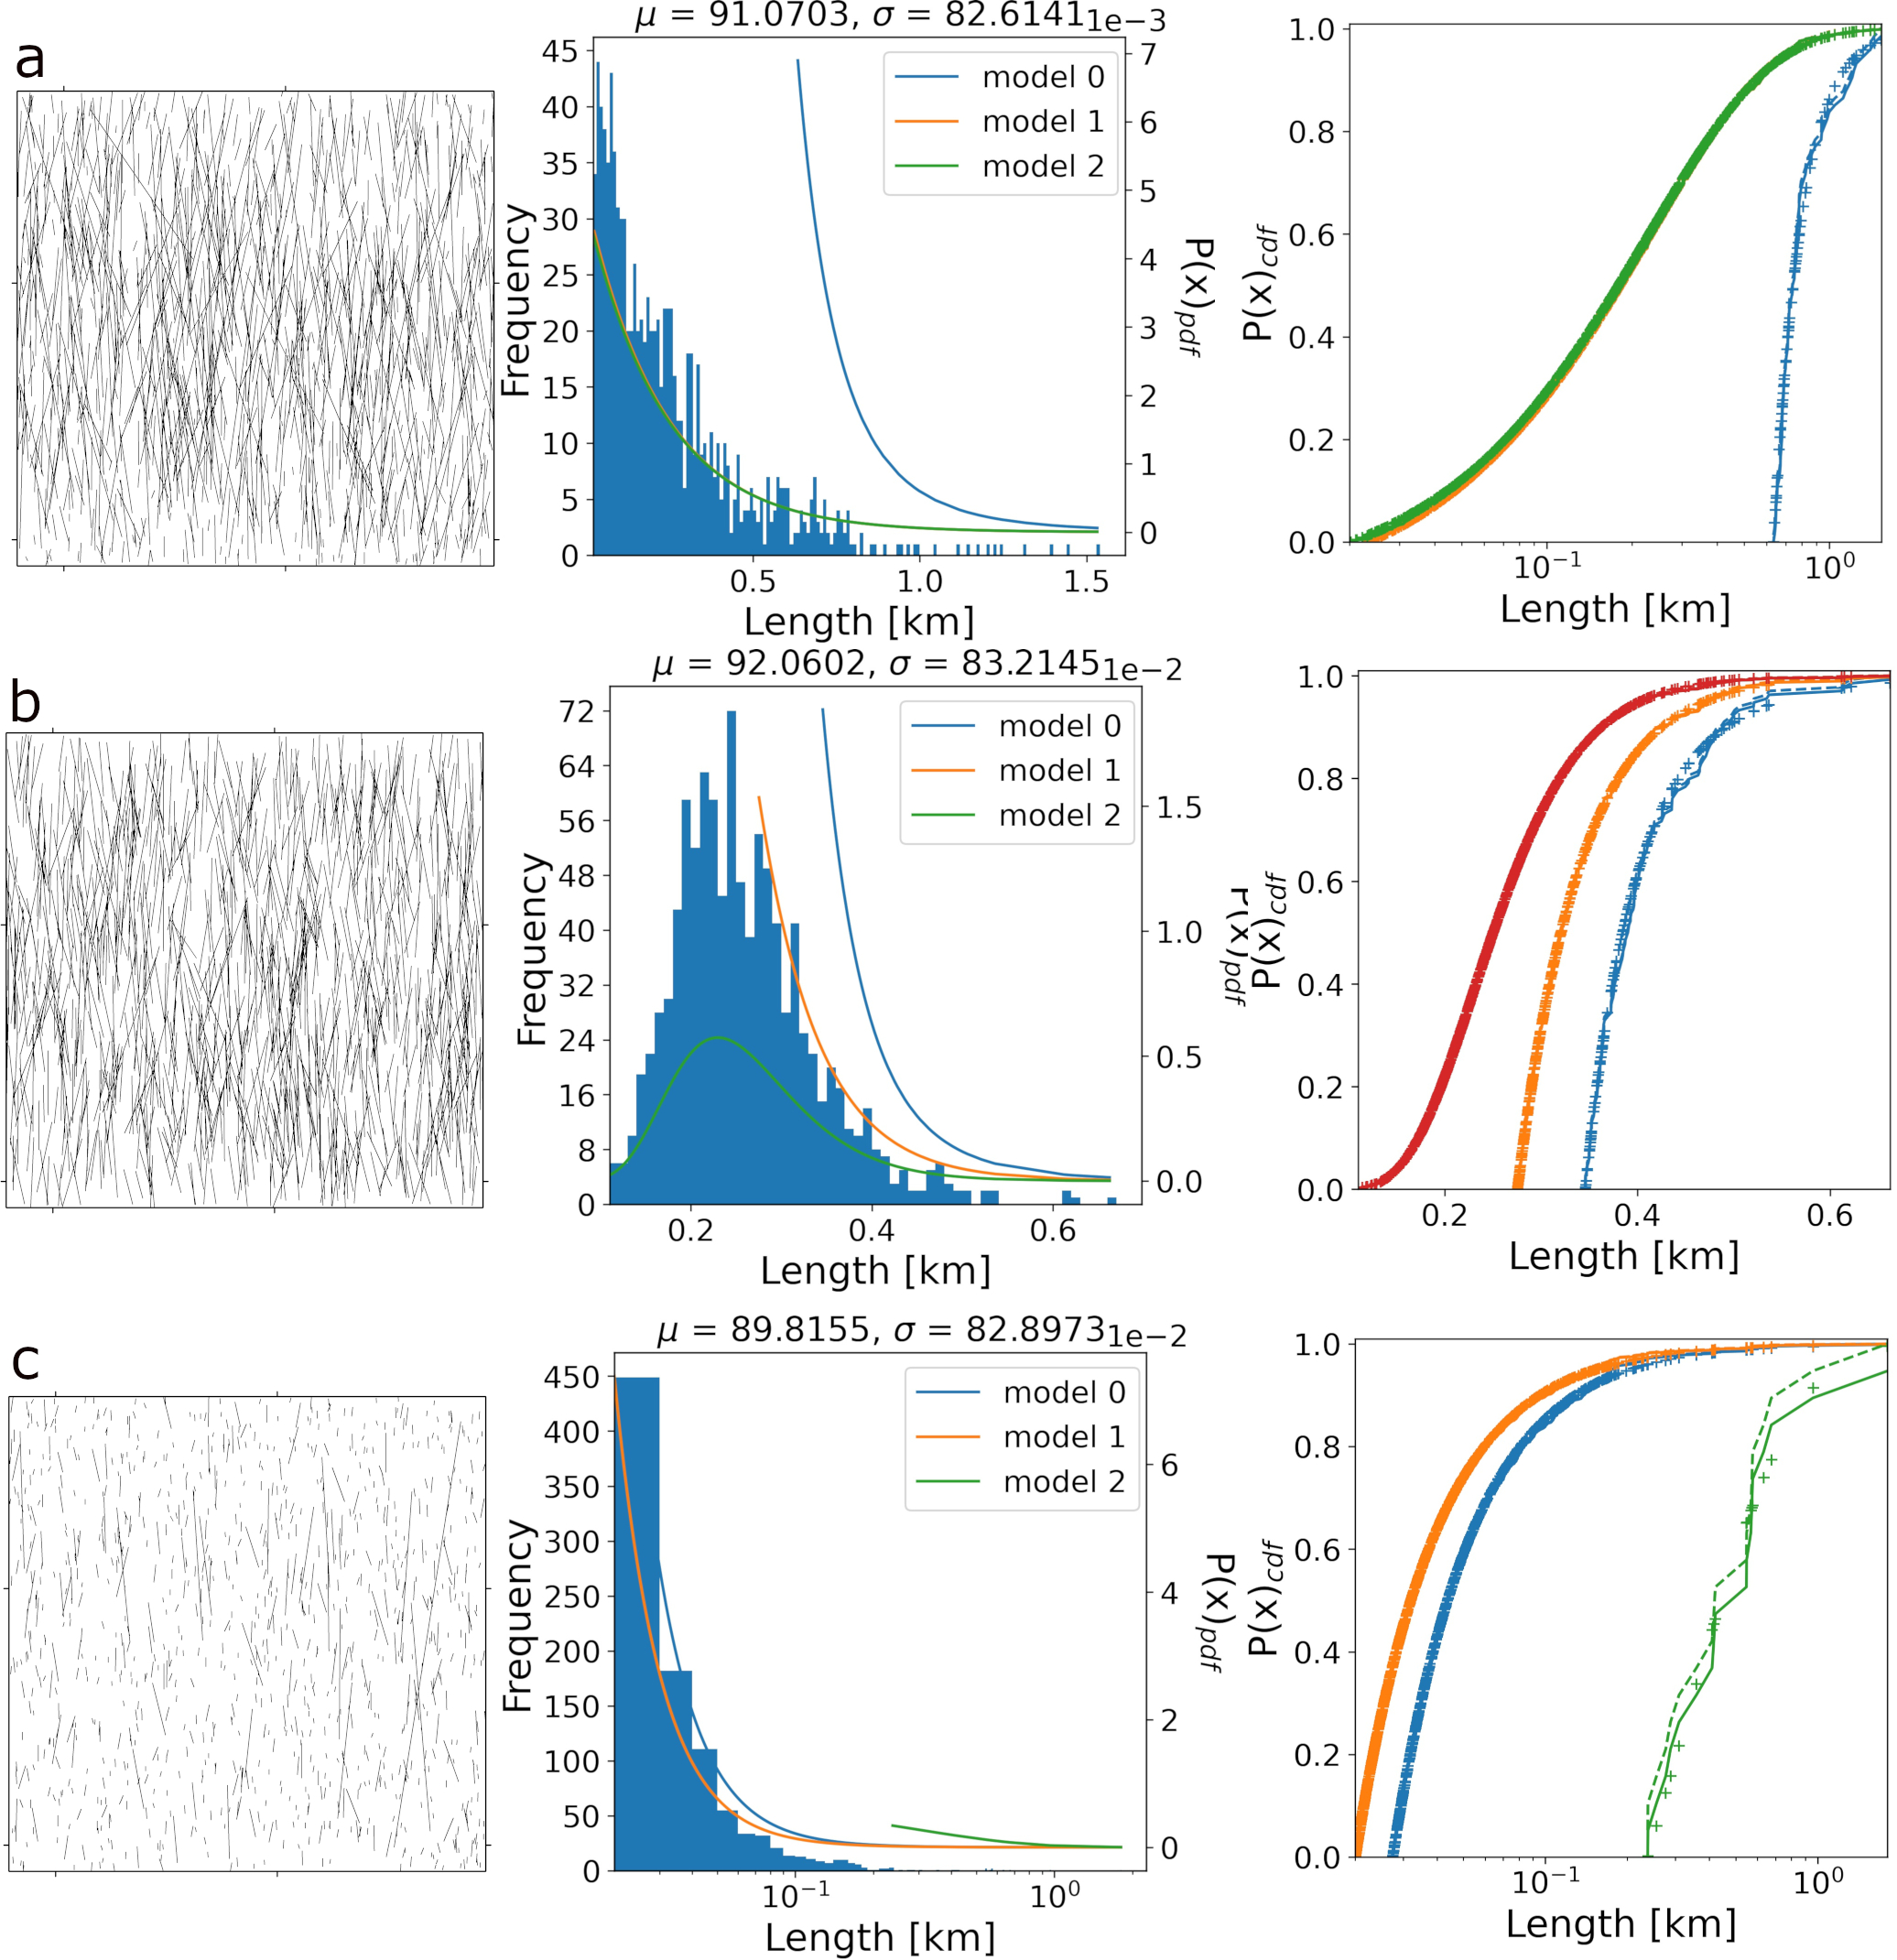
\includegraphics[width=8.5cm]{fig02.jpg}
	\caption{Example of fitting exponential, log-normal, or power law models to synthetic data comprising 1000 lineaments whose length follow one of the three distributions. In each row of this figure the synthetic data (right), the probability density functions of the models compared to the histogram (centre), and the cumulative distribution functions of the models are shown. \\
\textbf{a} \textit{synthetic exponential}: Three models are fitted for different data ranges. Model 0 follows a power law distribution (c: 0.0067; $\alpha$: 5.373 above 634.139 m representing 74 lineaments. Model 1 follows a an exponential distribution with $\lambda: 0.00439$ for lineament longer than 23.1241m  representing  994 lines. Model 3 fits an exponential distribution to the complete data range with $\lambda$: 0.004367. \\
\textbf{b} \textit{synthetic log-normal}: Three models are fitted to different ranges of this randomly created dataset. Model 0 follows a Power law distribution with c: 00188 and $\alpha$: 7.5243 for lineaments longer than 345,705 corresponding to 134 of the 1000 lines. Model 1 fits an exponetnial model with $\lambda: 0.0153$ to to all lines longer than 275.256 which are 374 lines. Model 2 represents a log-normal model with $\mu:$ 5.521 and $\sigma$: 0.29 for the entire range of lines in the dataset.  \\
\textbf{c} \textit{synthetic power-law}: Three models are fitted to this synthetic dataset. Model 0 represents a power-law fit with c: 0.0544 and $\alpha$: 2.493 for lines longer than 27.4332 which are 639 of the dataset. Model 1 fits a power-law distribution to the entire range of teh model with parameters c: 0.0738 and $\alpha$: 2.477. Model 3 represents an exponential fit to lines above 237.597 which are 19 of the total 1000.}
\label{fig02}
\end{figure}

\subsection{Box-Counting dimension}
The ``Minkowsi-Boulingard'' dimension is determined via box counting. For a detailed description of the box counting method in fracture networks we refer to~\citep{Roy2017}.  We will briefly outline our implementation of the box-counting algorithm, by utilising quad trees.
The maximum scale is represented by boxes with a side length equal to the longest lineament in the set whereas the smallest scale is derived from an arbitrary (user-defined?) number of recursions. During each recursion the area covered by each box is quartered.
The maximum scale is represented by boxes with a side length equal to the longest lineament in the set whereas the smallest scale is derived from an number of recursions. During each recursion the area covered by each box is quartered.

\begin{figure}[h]
\centering
	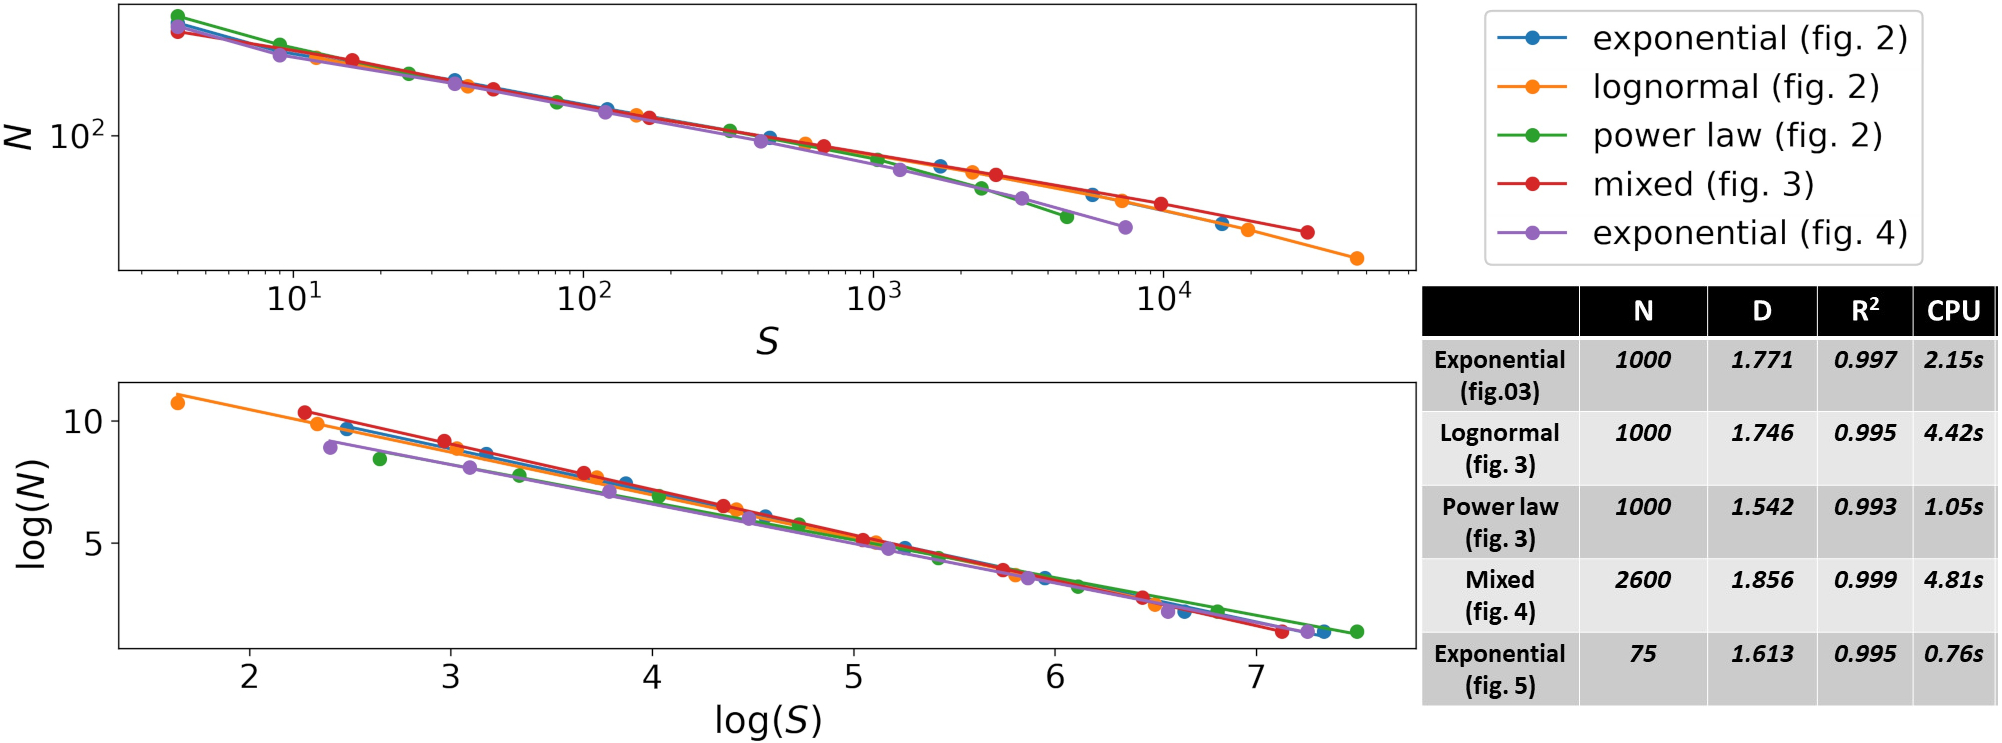
\includegraphics[width=8.5cm]{fig03.jpg}
	\caption{Results of the box counting for some of the synthetic networks shown in this manuscript. As the maximum and minimum box size is related to the largest and smallest feature in the data set, the computational time is not only a function of the total number (density) of entities but also strongly depends on the range of the feature length. Due to the implementation of the quad-tree method computational time is highest for data that fills the area of interest. }
\label{fig03}
\end{figure}

The first layer of boxes is created, covering the entire bounding box. Note that the origin of these covering boxes may be iteratively offset to evaluate the uncertainty of the fractal dimension. In the next step, the number of non-empty boxes (\textit{n}) it determined. At each scale, where a lineament overlaps a box, that box is marked as filled, and we compare the lineament against that box's four quadrants. When a lineament overlaps with a quadrant, the comparison is performed recursively using the quadrant and the portion of the lineament that overlaps with that quadrant. This recursive refinement is performed until the minimum scale is reached. In this manner, the count of non-empty boxes is obtained for different sizes. For each scale, we record the side length of the boxes (s) and the number of boxes that are filled (\textit{n}). We use least-squares fitting to fit a line of $log(n)$ as a function of $log(s)$ and report its slope as the fractal dimension. (TODO: double-check what we do with the box counts after they are reported.)


\subsection{Principal Orientations}\label{principal_orientations}
The orientation of a lineament is calculated from the lineament tips. The angle of orientation is expressed as a value between 0$\deg$ and 180$\deg$. This data can be used to distinguish different lineament sets and identify major structural trends in an area. An estimated probability density function (\textit{epdf}) of the angle distribution is produced using Kernel Density Estimation (\textit{KDE}, \textbf{table 1}), with a Gaussian kernel. We attempt to fit a multiple Gaussian to the \textit{epdf} by first attempting to fit between one and ten gaussians. For each number of Gaussians, we calculate the Akaike Information Criterion (\textit{AIC}), and choose the number of Gaussians that results on the lowest \textit{AIC}. The non-linear function fitting algorithm from the GSL is used to fit each number of Gaussian to the epdf. The initial parameters for the fitting are determined from the inflection points of the \textit{epdf}. We create pairs of falling, then the next rising, zero-crossings its second derivative. For each pair, the position is set as the mid-point of the two crossings, the amplitude is the value of the \textit{epdf} at that position, and the width is set as the distance between the zero-crossings. If we find more pairs of zero-crossings than the number of Gaussians we are currently trying to fit, the \textit{epdf} is increasingly smoothed until it has the desired number of crossings. This smoothing is reset for each number of Gaussians. If the number of crossings we find is equals to the number of Gaussians we are currently evaluating, then we calculate the residual between the epdf data and the pdf modelled by the fitted Gaussians and use this residual as the pdf data when trying to fit greater numbers of Gaussians. If we are still unable to find additional pairs of inflection points after calculating the residuals, then we stop trying to fit additional Gaussians and only consider the values that we have already fit.
\begin{equation}
\hat{f}(x) = \frac{1}{n}\sum\limits_{i=1}^n K_h (x-x_i) = \frac{1}{nh}\sum\limits_{i=1}^n K\frac{x-x_i}{h} \\
 K =\frac{1}{\sqrt{2\pi}}e^{\frac{x^2}{2}} \\
 \int h_h(x)dx = 1
\end{equation}

\begin{figure}[h]
\centering
	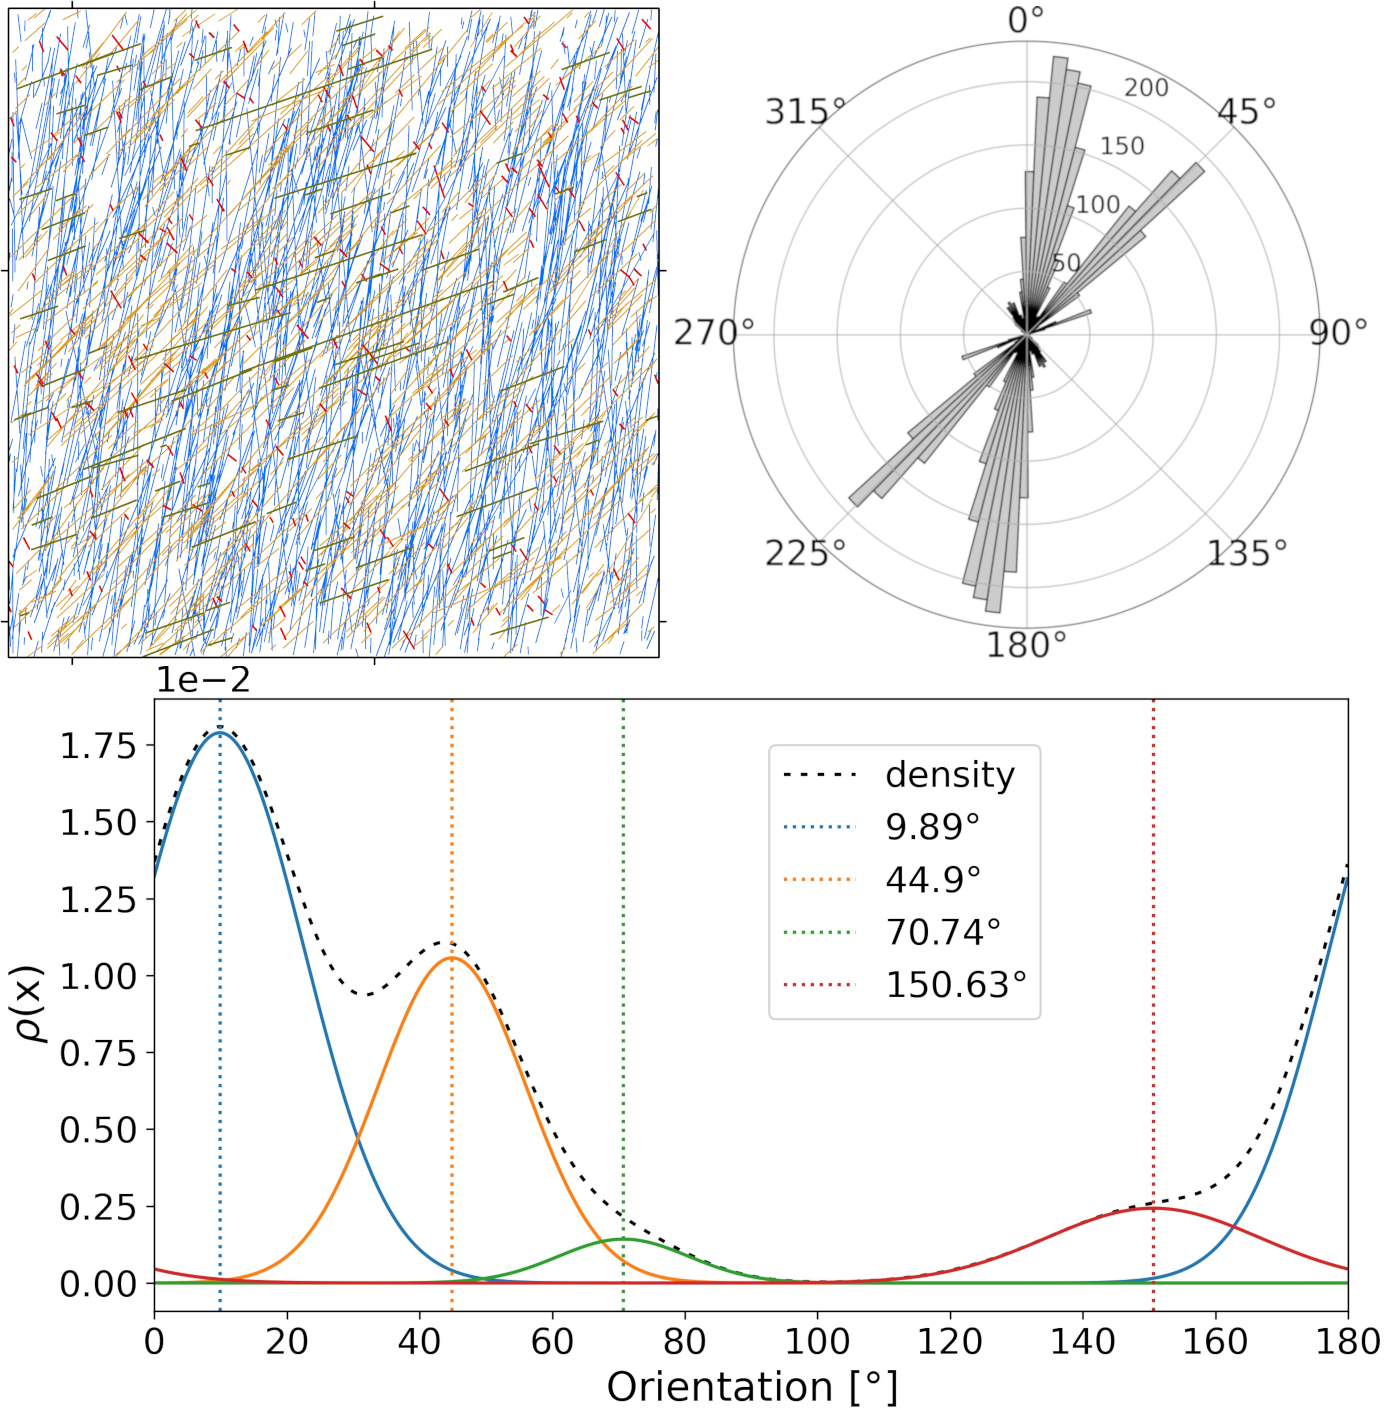
\includegraphics[width=8.5cm]{fig04.jpg}
	\caption{Example of fitting Gaussian models to a synthetic dataset comprising 2600 features that are generated for four different directions with variable numbers and variances. The principal directions visible by in the rose diagram can automatically be obtained via iteratively fitting models comprising different numbers of Gaussian, the amplitude of the Gaussian correspondent to the number of lines that fit into this distribution. Note that in lower plot of this figure the areas below the Gaussian is chosen to add up to one and the area of each Gaussian represent the frequency of the elements belonging to the particular Gaussian.}
\label{fig04}
\end{figure}

\subsection{Sinuosity}
The sinuosity is defined as the ratio between the length of a feature and the geometrical distance between its end points. 

\begin{table}[width=.75\linewidth,cols=2,pos=h]
\caption{Geometric parameters derived during the analysis. .}\label{tbl01}
	\begin{tabular*}{\tblwidth}{@{} LC@{} }
		\toprule
		Parameter & Expression\\
		\midrule
		Sinuosity ($s$) 			& $s = \frac{D}{L}$\\
		Orientation ($\alpha$) 		& $\alpha = atan\left( \frac{x_1 - x_2}{y_1 - y_2} \frac{180}{\pi} \right)$\\
		Orientations ($Nb$) 		& $Nb = \forall x: f'_h(x) = 0 \land f''_h(x) < 0 $\\
		Length distribution ($_d$) 	& $R = sum ln \left( pdf_a(x) \right) - l \left( pdf_b(x) \right) $ \\
									& $\sigma = \sqrt{\frac{1}{N} \sum \left( \left( ln(pdf_a(x) \right) - \left( pdf_b(x) \right) - \frac{R}{N} \right)^2}$\\
		Density  					& $P_{10} = \frac{N}{L}; P_{20} = \frac{N}{A}; P_{20_c} = \frac{N}{2\pi r^2}$\\
		Intensity  					& $S = \frac{1}{P_{10}}; P_{21} = \frac{\sum l}{A}; P_{21_c} = \frac{\pi r}{2} \frac{n}{m}$\\
		\bottomrule
	\end{tabular*}
\end{table}

\section{Spatial arrangements}
With spatial arrangement we refer the density or length per unit area, the Minkowsi-Boulingard dimension, and the topology.

\subsection{Density, Intensity, and Spacing}
The characterization of the networks in terms of density, intensity, and spacing can be performed either with scan lines or through window sampling~\citep{Zeeb2013, Watkins2015, Sanderson2019}. With these sampling methods the relative abundance of fractures can be expresses as density (\textit{P}), spacing (\textit{S}) or intensity (\textit{I}). Based on the sampling method, linear intensity ($P_{10}$) is obtained though line scan sampling and lineament intensity (P20) and length intensity (P21) are obtained from window sampling.

\subsubsection{Scanline sampling}
The metrics obtained by scanline sampling are the average spacing ($\overline{S}$) and the liner intensity ($P_{10}$). In order to minimize the sampling bias, numerous scanlines need to be analysed that are oriented perpendicular to the principal orientations of the analysed features. Therefore, scanline sampling in FracG can only performed if the principal orientation were obtained (see section~\ref{principal_orientations}). The start points of the sampling lines are randomly chosen within the convex hull of the domain. This ensures that the analysis is focused on the areas comprising features while omitting void areas. The orientation of the scanline by randomly choosing a orientation that is perpendicular to one of the principal orientations. This minimizes orientation dependent bias of scanline sampling to some extend but cannot address bias caused by truncation or censoring effects that would already be present in the initial data.
Intensity ($P_{10}$) and average spacing ($\overline{S}$) are calculated as:

\begin{equation}
	P_{10} = \frac{I}{L} \\
	\overline{S} = \frac{l}{I-1}
\end{equation}

Where $I$ is the total number of intersection, $L$ is length in m, and $l$ is the distance between to consecutive points along the scaline. For every scanline the underlying principal orientation, the start- and endpoint coordinates, length, number of intersections, intersection intensity ($P_{10}$) and the average spacing are reported in a table. 
The user can define the total number of scalines and the desired spacing between lines of the same orientation. For large sample-line numbers FracG will attempt to fill the domain with lines that are close to the horizontal extend of the rectangular area while maintaining the predefined minimum spacing. After each failed attempt of constructing a line either the minimum length of the scanline or the minimum spacing is reduced. If after $1e^5$ failed attempt to construct a line, the program will terminate.

In figure~\ref{fig05} we show 50 scanlines generated for a synthetic dataset comprising two principal orientation following an exponential length distribution.

\begin{figure}[h]
\centering
	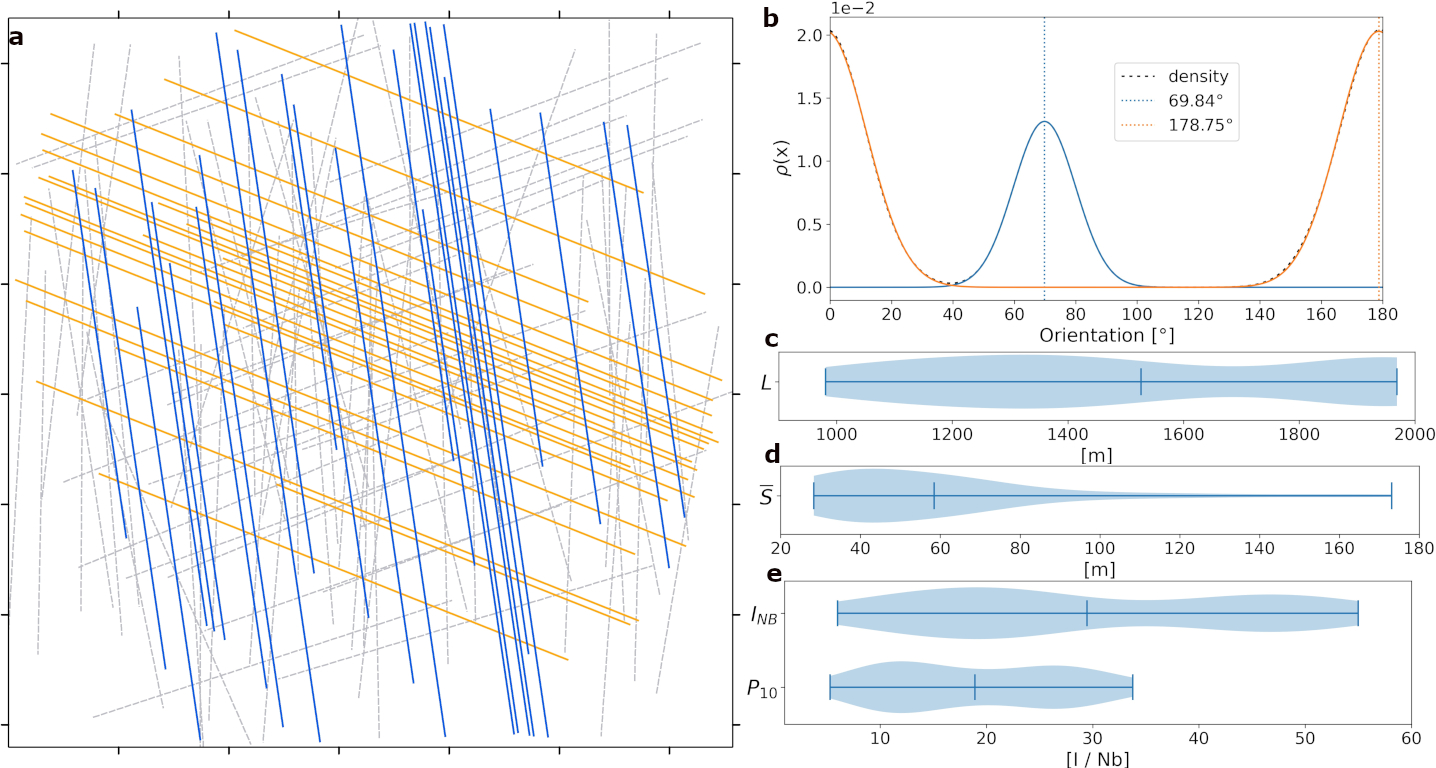
\includegraphics[width=8.5cm]{fig05.jpg}
	\caption{a 50 scanlines that were randomly created following a uniform random distribution. The two sets of sample lines are constructed perpendicular to one of the principal origination that were obtained via fitting Gaussians to the KDE. c shows the length distribution of scanlines, d shows the distribution of average spacing, and e shows the intersection numbers and linear intensities of the 50 scanlines. }
\label{fig05}
\end{figure}

\subsubsection{Window sampling}
Rectangular Window sampling is performed for obtaining density (total number, $P_{20}$), intensity (cumulative length, $P_{21}$), and distances per unit area for the domain. Two types of distance maps are created: the minimum distance of every pixel centre to the nearest line, and the distance to the nearest line centre. 
Every sampling window is a pixel in the created raster file whereas the window or pixel size can be defined by the user and is initially set to 1000m by 1000m. For a better visulaization reampling to a 10$^th$ of


In figure~\ref{fig05} we show the four maps types obtained for a synthetic networks comprising 75 elements (same networks as in figure~\ref{fig04}. The left image column show the data created by window sampling with a pixels size of . 


The right a map is re-sampled to a pixel size of one 10$^{th}$ of the window size using cubic B-spline approximation with a 4 by 4 kernel interpolation. Note that the pixel values are projected back to the initial range after re-sampling to avoid unnatural odd number for instance for the density maps.

\begin{figure}[h]
\centering
	\includegraphics[width=8.5cm]{fig06.jpg}
	\caption{Examples of spatial analysis performed on a synthetic dataset comprising 75 lines with two dominant orientations. The greyscale images represent the results of rectangular window sampling and the coloured maps show the results after up-sampled by one order of magnitude. \textbf{a} density map showing intersections per pixel, \textbf{b} intensity displaying cumulative length of lines per pixel, \textbf{c} distance map of pixel centres to nearest line, and \textbf{d} distance map of pixel centres to nearest line centre.}
\label{fig06}
\end{figure}


\section{Topological Analysis}
We follow the approach described by~\cite{Sanderson2018, Sanderson2019} to obtain the topology metrics from a georeferenced graph. This data structure can be linked to raster data and utilized for assessing additional network properties by applying graph algorithms. In a 2D projection, the system can be presented as a set of vertices and edges. This graph yields information on geometry as well as on topology and allows for characterization of the network in terms connectivity and percolation~\citep{Manzocchi2002, Nixon2013, Sanderson2015, Sanderson2018}. For the graph representation the vertices are labelled depending on the number of edges incident with this vertex, called the degree of the vertex. Three different degrees of vertices exist: isolated tips (1), junctions (3), and crossings (4). Even if the fault traces are not connected at the surface, a hydraulic connectivity between neighbouring faults might exist through the fault damage zone (figure 2 a). Damage zone geometries differ depending on the location relative to (distance from…?) the fault core~\citep{Peacock2017}. Along a single fault the overall fracture density in the wall damage (zone?) (Wdz) and tip damage zone (Tdz) will have different geometries and fracture densities. In a fracture network, damage zones at junctions (Ydz) or crossings (Xdz) will comprise higher fracture densities. Via linking damage zones (Ldz) a hydraulic connectivity between neighbouring faults can be established even if the 2D fault traces do not intercept. 
The lineaments are converted into an undirected adjacency list with bundled properties (maybe rephrase, in order to focus on what is important to the reader).  Geographic coordinates of the edges (line strings) and the vertices (points) are directly assigned to graph. The next step is to locate the intersection points of the lineaments, split the traces at these intersection points, and add vertices at these intersections. After this splitting but before the graph’s analysis, the isolated tips whose lengths are below a defined threshold will be removed from the graph. This ensures that y-intersections are not falsely interpreted as x-intersections. Our framework accounts for this by defining a minimum distance threshold, where lineaments that are within this distance of each other are considered to intersect even if they do not overlap.

\subsection{Graph representation}
At the beginning of the analysis the consistency of the created graph is tested via Boyer-Myrvold Planarity Test. This test ensures that the network geometry is captured correctly, and Euler's formula applies. Subsequently, the graph and connected components comprising at least a certain number of edges that can be defined by the user (this sentence is incomplete). The percolation state can be evaluated in a tertiary diagram (MANZOCCHI, 2002) by utilizing the reported values. The weights assigned to the edges are the geographical length allowing for further spatial investigation of the network. The area that is occupied by the network is determine by the convex hull around the graph which minimized the bias for area-dependent calculations, such as line and branch frequency. The parameters derived from the graph analysis are reported as a tab-separated text file and are summarized in table~\ref{tbl02}. 

\begin{table}[width=.75\linewidth,cols=2,pos=h]
\caption{Parameters obtained from the graph. Number of line tips (NI), number of Y-nodes (NY), number of X-Nodes (NX), branch types: IX, IY, II, YY, XX, number of lines (NL), length of branch( lb), area of convex hull around graph (A), node degree (deg(v)).}\label{tbl02}
	\begin{tabular*}{\tblwidth}{@{} LL@{} }
		\toprule
		Parameter & Expression\\
		\midrule
		Number of Vertices ($N_v$)				& $N_v = N_i + N_y + N_x$\\
		Number of Branches ($N_b$)				& $N_B = IX + IY + YX + YY + XX + II$\\
		Connecting Nodes ($N_c$)				& $N_c = NX+NY$\\
		Average Branch Length ($\bar{l_B}$) 	& $\bar{l_B} = \frac{\sum\limits_{i=0}^n l_{B_i}}{N_B}$\\
		Connecting Node Frequency ($f_{Nc}$)	& $f_{NC} = \frac{\sum N_y + \sum N_x}{N_v}$\\
		Dimensionless Intensity ($B_{22}$) 		& $B_{22} + P_{21} \bar{L_B}$\\
		Average degree ($deg_{av}$) 			& $deg_{av} + \frac{\sum deg{v}}{N_v}$\\
		Average connection per line ($C_{av}$)	& $C_{av} = \frac{2N_x + N_y}{N_v}$\\
		Number of faces ($f$) & $ f = 2N_v+N_B$\\
		\bottomrule
	\end{tabular*}
\end{table}

\begin{figure}[h]
\centering
	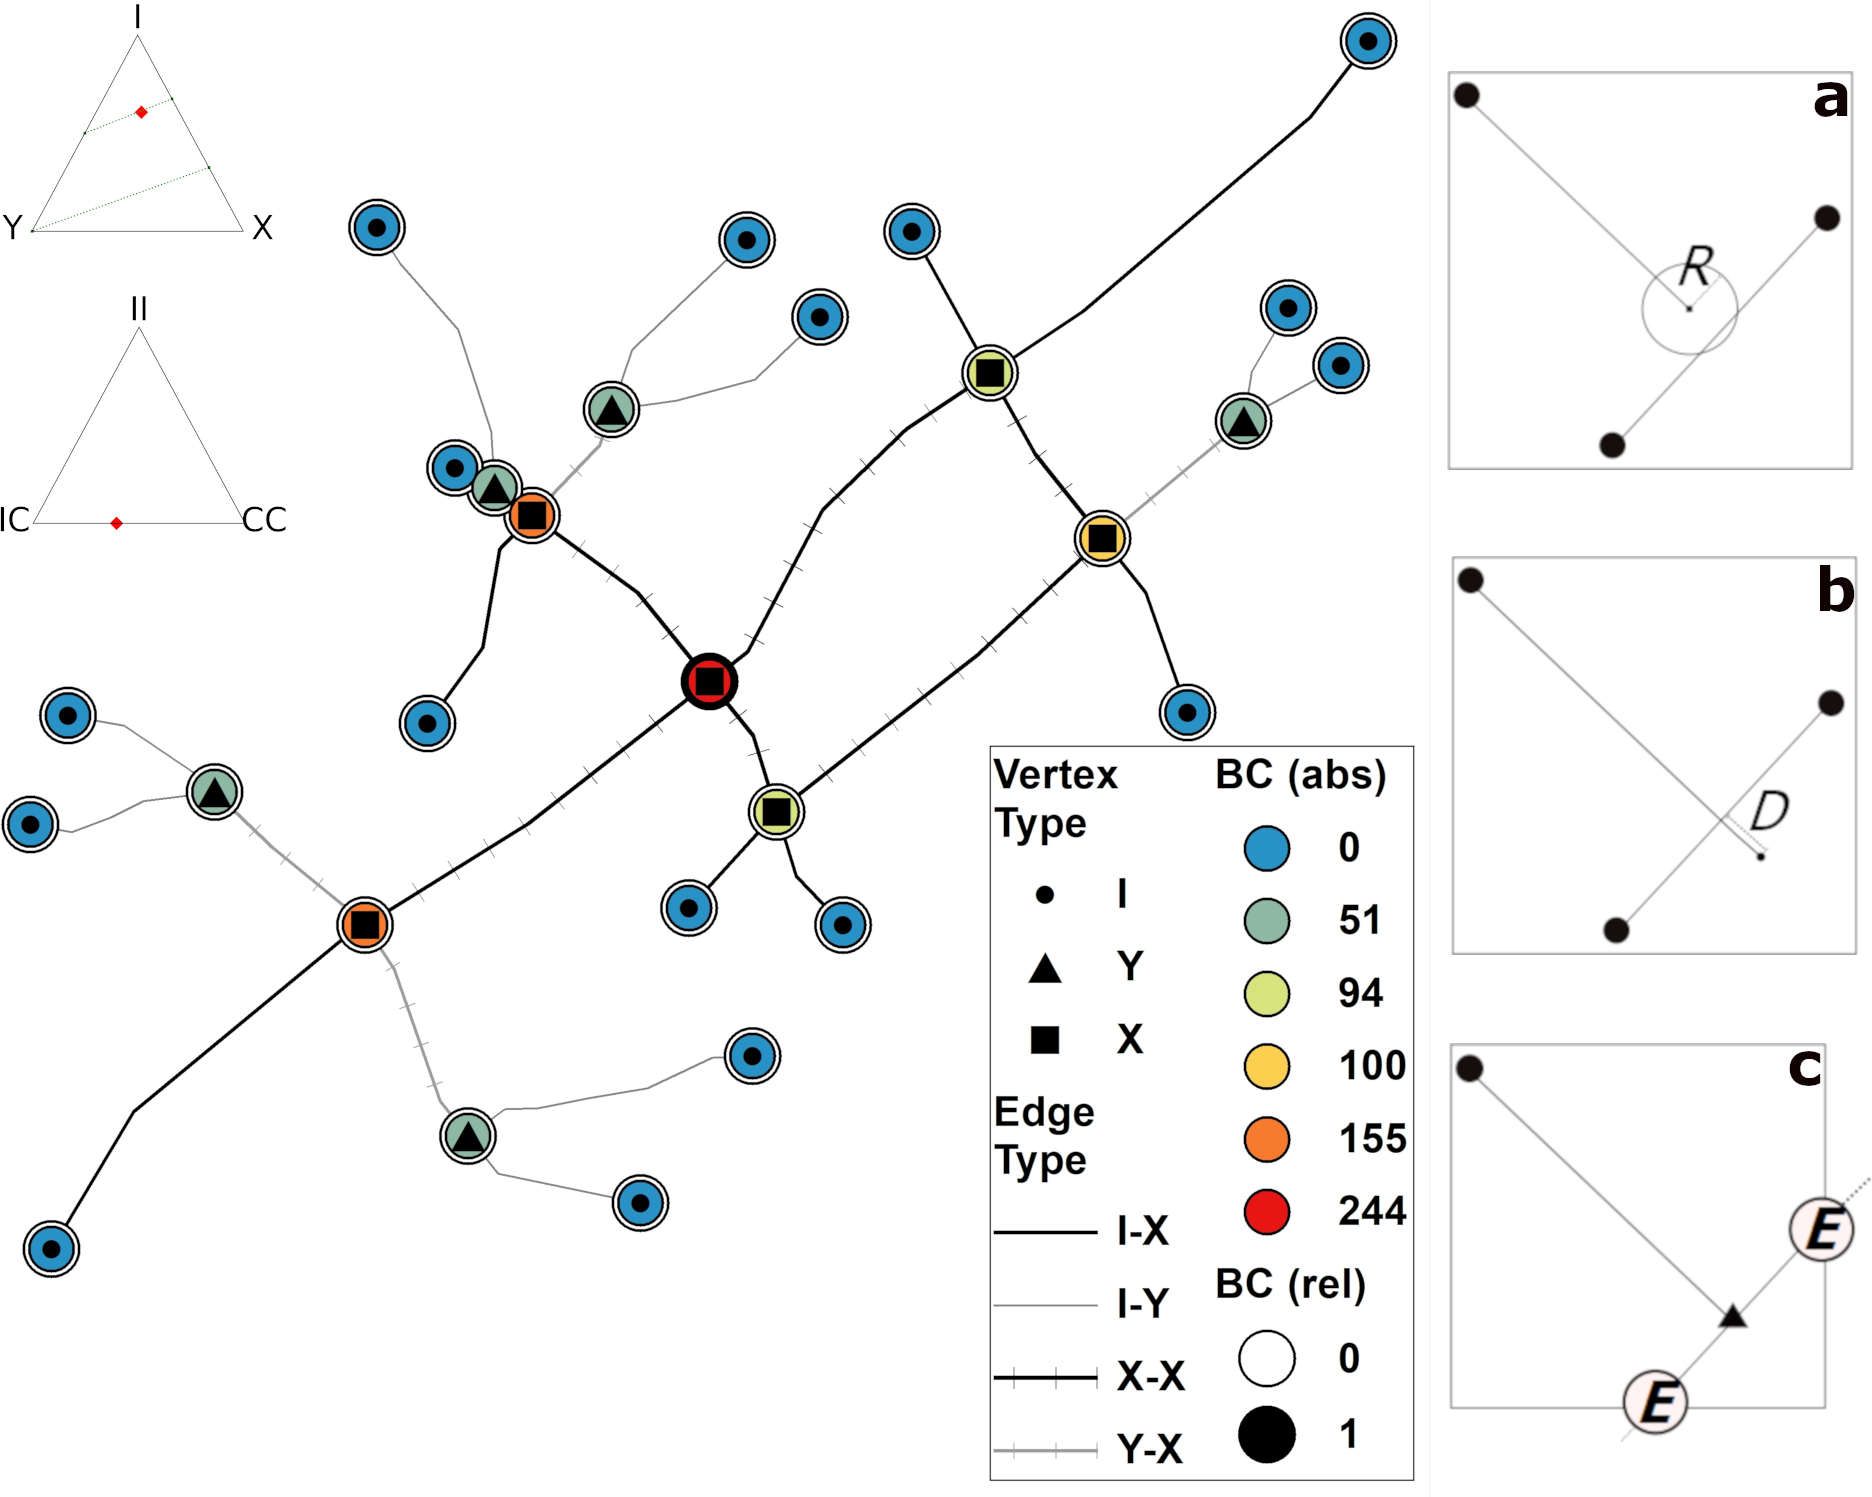
\includegraphics[width=8.5cm]{fig07.jpg}
	\caption{Example of a networks graph representation. Vertex types are labelled according to the number of outgoing edges (I:1, Y:3, and X:4). The edge types classification is based on the vertices adjacent to each edge. The colour circles surrounding every vertex show the absolute betweenness centrality (BC (abs)) and the large black and white circles show the relative betweenness centrality (BC (rel)). The two ternary plots in the upper right represent the network classification based in vertex type (I-Y-X) and based on edge connectivity (II-IC-CC). The two dotted lines in the upper ternary plot represent the average degree of vertices in a network that is related to the percolation threshold.\\
	To the three important parameters fro building a georeferenced graph are shown schematically. \textbf{a} critical merging distance which is a buffer around each isolated vertex. If an edge is located within this buffer the edges are merged. \textbf{b} critical length governing the removal of spurs that would lead to falsely classifying a vertex as X-node instead of Y-node. \textbf{c} if a graph should be cropped to a area of interest (aoi) (i.e. the extend of a raster file) some features will be truncated along the boundaries of the aoi. To minimize the truncation bias fro statistical analysis cause by the clipping, the intersection points between line features and bounding box are labelled as edge nodes (E-nodes). Vertices labelled as E-nodes are exuded from any analysis and so are edges that contain an E-node.}
\label{fig07}
\end{figure}

\subsubsection{Graph Algorithms}
graph analysis that are allied for obtaining more topological information about the networks are minimum spanning tree, shortest path, and betweenness centrality. We consider solving maximum flow as a separate problem and describe this in greater detail in the subsequent section.

A spanning tree is a tree structure that maintains the overall connectivity of the vertices. A single undirected graph can have several of such structures whereas the minimum spanning tree is one with the lowest sum of edge weights. 

The shortest path algorithm is applied to a weighted undirected graph where the edge weights can either be the length of the edge, the centre value, the mean value of the edge, or the profile along the edge. The algorithm we utilize is the Dijkstra Shortest Path from the boost graph library.


\begin{figure}[h]
\centering
	\includegraphics[width=8.5cm]{fig08.jpg}
	\caption{}
\label{fig08}
\end{figure}

\subsection{Maximum Flow}
We utilize the ``Boykov-Kolmogorov Maximum Flow algorithm'' of the boost graph library which requires teh creation of a directed graph with two directed edges for each undirected edge. The value associated with each directed edge is the maximum capacity of fluid flow between its start and end vertices, in each direction of its corresponding undirected edge (this could be phrased better). We implemented three different functions to derive edge capacities based on their length, orientation, or a combination of length and orientation. The direction of the flow is derived from vertex weights of an edge as the flow is always from high to lower values, taking also into account that the flow cannot reach higher than the source vertex.  


The vertex weights (we’re not really using these as ``weights'', maybe we should call them the height of each vertex) can either be derived from a raster file (e.g. DEM) or from horizontal or vertical gradients (I need to check what we’re doing here – I’ve only seen using  raster file as a DEM, and in any case those gradients will also come from a raster). The maximum and minimum values of the gradients must be defined by the user and a liner (is this the correct word?) gradient between the two values is generated in the envelope around the graph (is the envelope around the graph or the edge? Also, if it is around the graph, call it the ``region of interest'' to be consistent with what is said above about using a raster file). 
The capacities are derived as described in table~\ref{tbl03}.

\begin{figure}[h]
\centering
	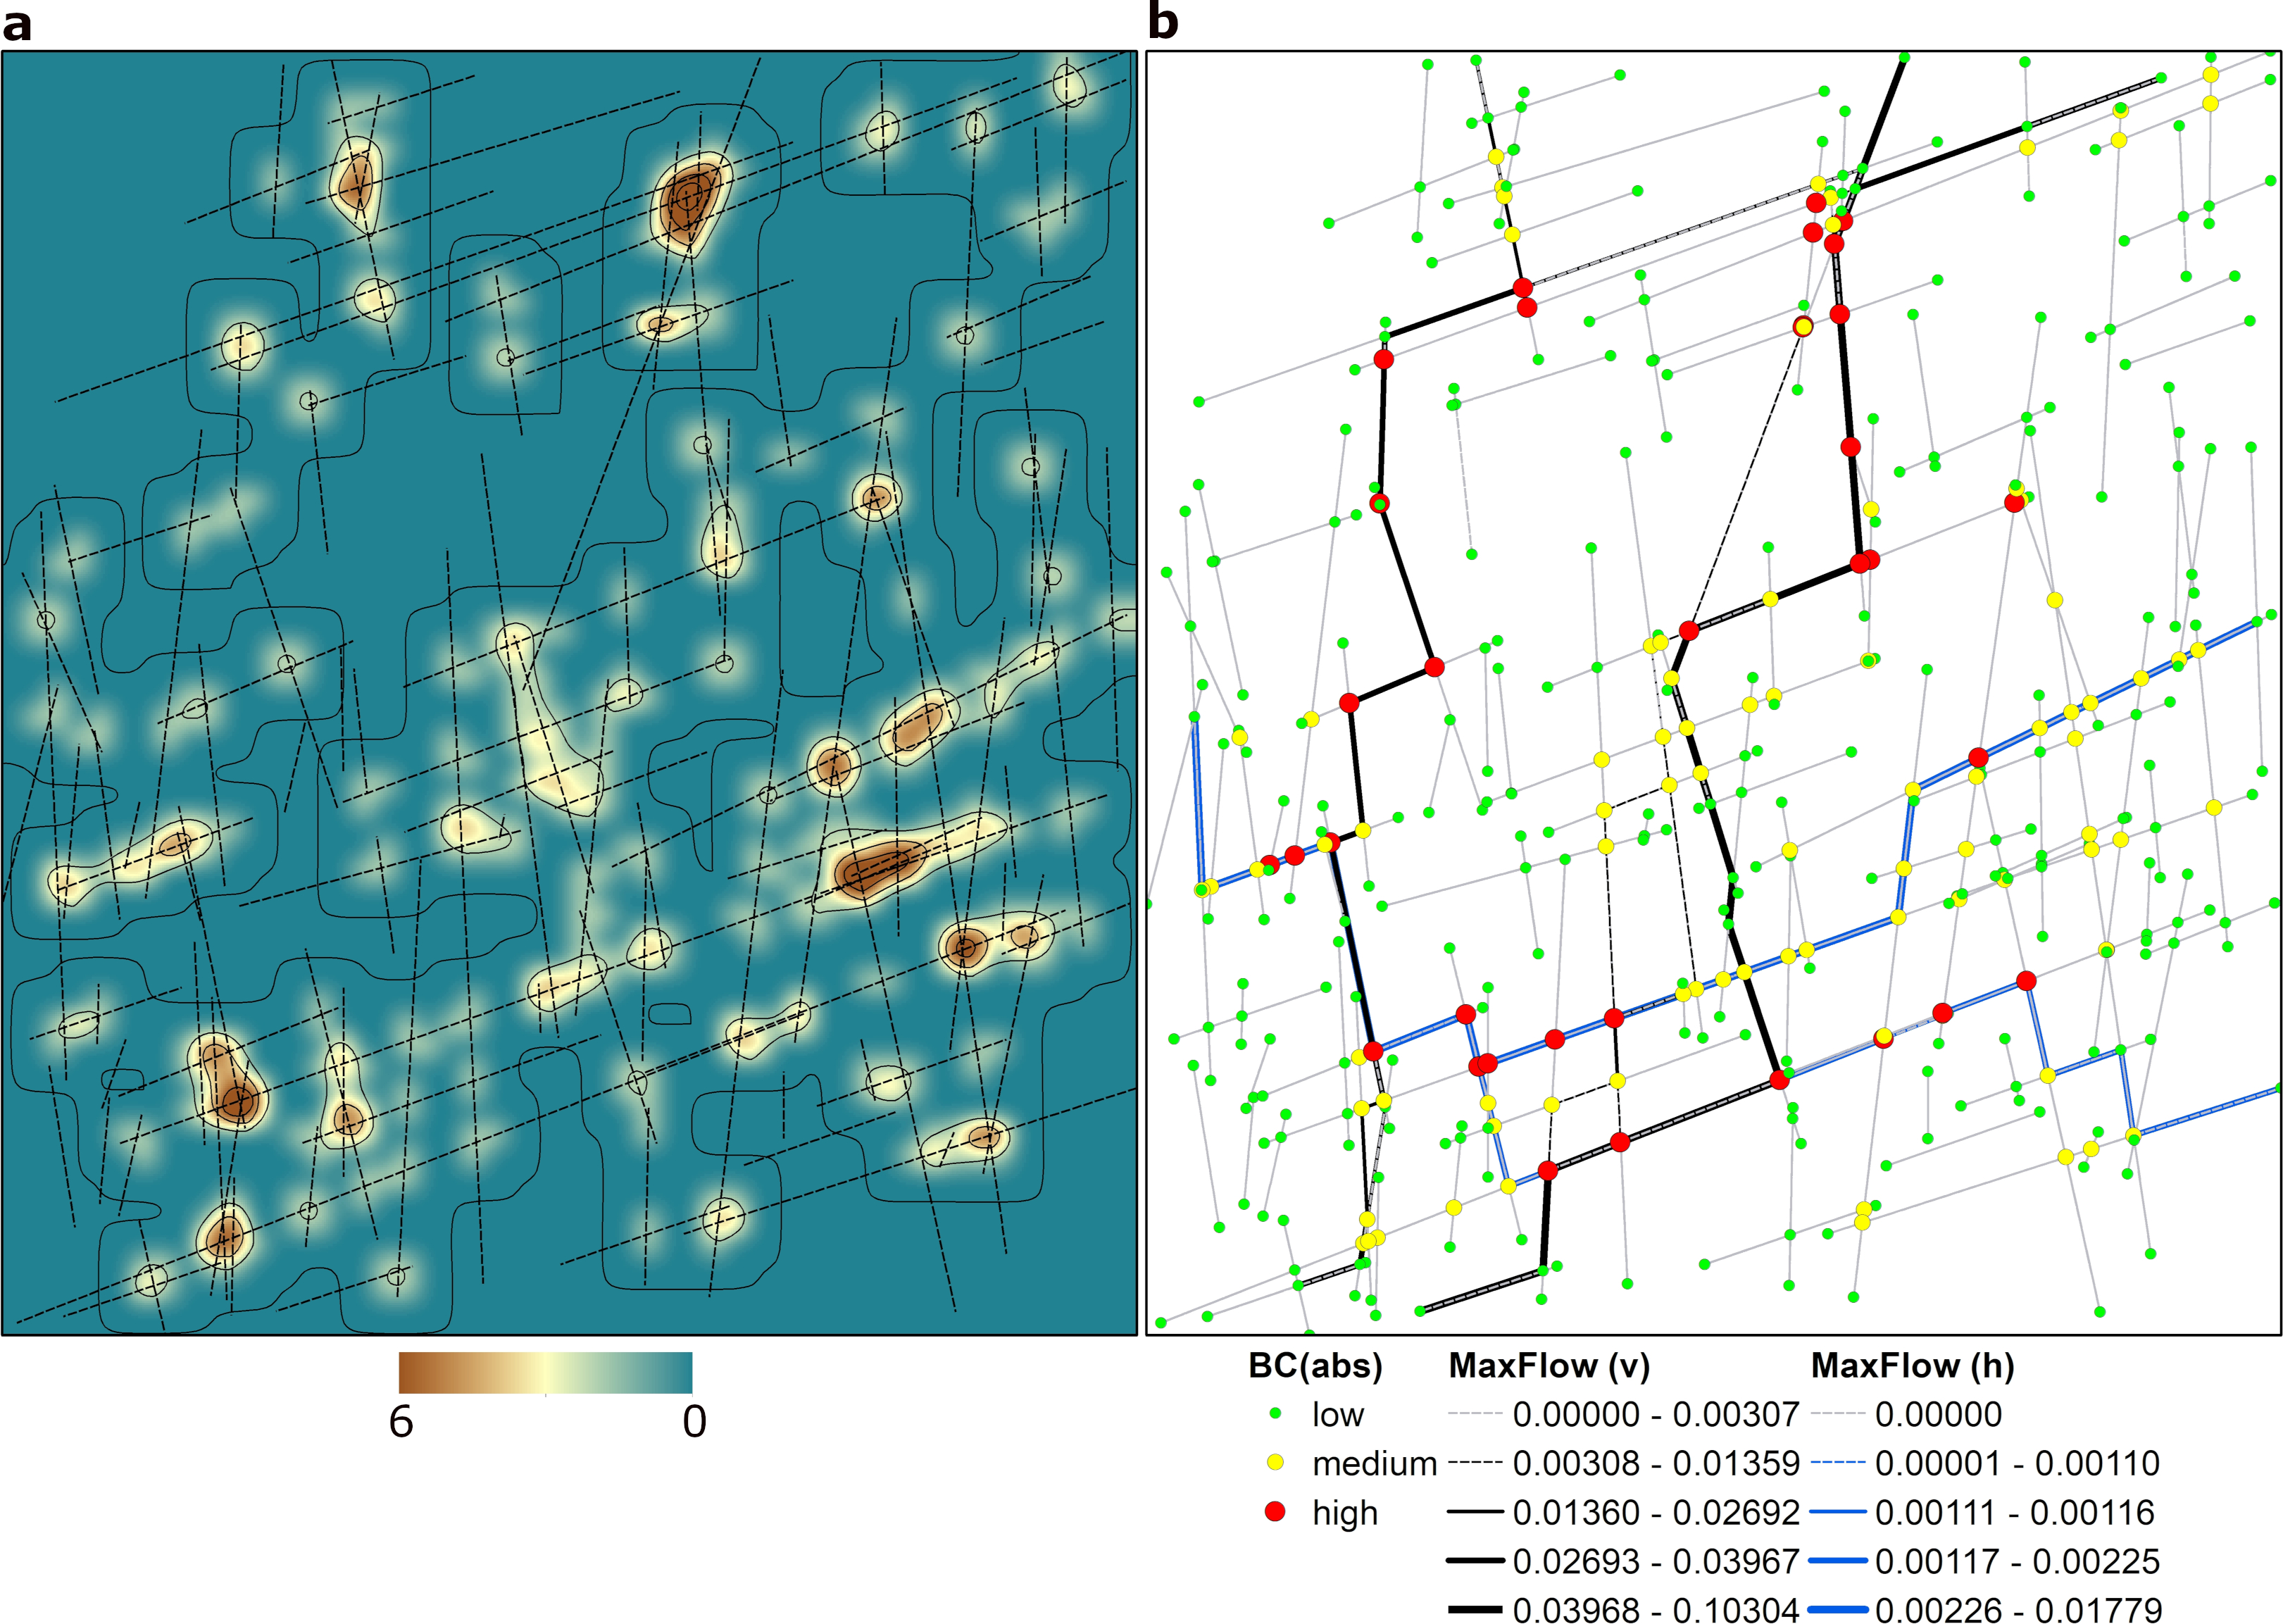
\includegraphics[width=8.5cm]{fig09.jpg}
	\caption{}
\label{fig09}
\end{figure}


\begin{table}[width=.75\linewidth,cols=2,pos=h]
\caption{Parameters obtained from the graph. Number of line tips (NI), number of Y-nodes (NY), number of X-Nodes (NX), branch types: IX, IY, II, YY, XX, number of lines (NL), length of branch( lb), area of convex hull around graph (A), node degree (deg(v)).}\label{tbl03}
	\begin{tabular*}{\tblwidth}{@{} LL@{} }
		\toprule
		Capacity dependency & Expression\\
		\midrule
		length  ($cap_l$) 					& $ cap_l = \frac{\kappa_f \sqrt{l}}{\frac{1}{2}\kappa_m l}$\\
		orientation  ($cap_o$) 				& $cap_o = \frac{1}{\sigma \sqrt{2 \pi exp^{-0.5\frac{\alpha - \mu}{\sigma}}}} x 1000$\\
		length and orientation ($cap_{lo}$) & $cap_{lo} = cap_l cap_o$ \\
		\bottomrule
	\end{tabular*}
\end{table}

\section{Raster data}
The analysis can be extended by adding raster data sets to the vector data. The rectangular area of interest is defined by the extent of each raster file and noData values are set to 0. The general statistics of the raster data such as minima, maxima, mean, and standard deviation are reported in a csv file together with the pixel values along strike and perpendicular to strike at the centre of the lines. The length of the cross line is 2.5 pixel resolution and representing the sampling ($d_s$) distance utilized for most of the raster analysis.
 
Lineaments which cross the borders of the raster will be cut to the raster area and marked as edge-nodes (E-nodes). Lineaments containing an edge node will be excluded from the statistical analysis of lineament length. 

After generating a graph clipped to the extent of the raster file, the statistical topological analysis previously described will be performed only for the area contained in the raster. Note that the extent of the raster files that are added to the analysis do not have to be consistent, but the geographical projection must be the same for the vector and any raster data that is added.

The values of the raster file are stored as edge and vertex weights. Data is collected at every vertex, at the centre (centre of what?), and along each edge. In addition, the gradient across the centre of the edges, the mean gradient across the segments (profile) and the gradient along the branches (before I forget, do we formally state what our definition of a branch is?) is calculated. Each value is stored as an edge weight which allows for performing additional analysis on the graph (Need to double check this - each edge in a graph only has a single weight. If we use different weights in different places, then we should say that we store these properties, and mention below when each property is used as a weight). For instance, if the raster data is a digital elevation model (DEM), the path with the maximum topographic gradient can be calculated based on the maximum flow algorithm. 

FIGURE 10

\section{Automatic Meshing: 2D with local refinement}
A finite element mesh can be created from the vector data utilizing the open-source mesh generator gmsh.
to generate 2D meshes conforming to the discontinuity traces that are represented by side sets. Discretizing the features as side sets allows for applying a mixed dimensional approach where faults or fractures are represented by elements of a lower dimensional order compared to the domain they are hosted in~\citep{Poulet2021}. Mesh-refinement is a function of distance tot eh sidesets. 
FIGURE 11
\section{Example: Central Gawler Craton, South Australia}
FIGURE 12

\section{Conclusion}
\section{Discussion}
\appendix
\section{My Appendix}
Appendix sections are coded under \verb+\appendix+.

\verb+\printcredits+ command is used after appendix sections to list 
author credit taxonomy contribution roles tagged using \verb+\credit+ 
in frontmatter.

\printcredits

%% Loading bibliography style file
%\bibliographystyle{model1-num-names}
\bibliographystyle{cas-model2-names}
% Loading bibliography database
\bibliography{FracG-refs}
\end{document}